\documentclass[10pt]{article}

\usepackage[margin=0.8in, top=0.7in, bottom=0.7in]{geometry}
\usepackage{titlesec}
\usepackage{enumitem}
\usepackage{tikz}
\usepackage{hyperref}
\usepackage{microtype}
\usepackage{booktabs}
\usepackage{array}
\usepackage{fancyhdr}

\usetikzlibrary{shapes.geometric, arrows.meta, positioning, calc}

\titleformat{\section}{\normalsize\bfseries}{}{0em}{}[\titlerule]
\titleformat{\subsection}{\small\bfseries}{}{0em}{}
\titlespacing{\section}{0pt}{6pt}{3pt}
\titlespacing{\subsection}{0pt}{4pt}{2pt}

\pagestyle{fancy}
\fancyhf{}
\renewcommand{\headrulewidth}{0.4pt}
\fancyhead[L]{\footnotesize S26CS6.401 --- Software Engineering $\cdot$ Project 3 Proposal}
\fancyhead[R]{\footnotesize Date: 13 Mar 2026}
\fancyfoot[C]{\footnotesize\thepage}

\setlist[itemize]{leftmargin=*, itemsep=0pt, topsep=1pt, parsep=0pt}
\setlist[enumerate]{leftmargin=*, itemsep=0pt, topsep=1pt, parsep=0pt}
\hypersetup{colorlinks=false, pdfborder={0 0 0}}
\setlength{\parskip}{3pt}
\setlength{\parindent}{0pt}

\begin{document}

\begin{center}
  {\Large\bfseries DocPilot}\\[3pt]
  {\normalsize A Copilot-Inspired Multi-Model Document Intelligence Platform}\\[5pt]
  {\small Team NO: \texttt{38} \quad$\cdot$\quad Domain: \textbf{Productivity} \quad$\cdot$\quad S26CS6.401 --- Project 3 Proposal}
\end{center}
\noindent\rule{\linewidth}{0.8pt}\vspace{1pt}

%────────────────────────────────────────────────────────────────────
\section{Description of the Use Case}

Knowledge workers --- students, researchers, legal professionals, and analysts --- routinely manage large, multi-format document corpora: research papers, contracts, lecture notes, and reports. Existing tools such as ChatPDF or Adobe AI address only narrow slices of this problem: single-document Q\&A with no persistent memory, no cross-document reasoning, and no intelligence about which model to invoke.

GitHub Copilot demonstrated that inserting an AI-native \textbf{pipeline directly into the editing workflow} --- one that understands context, suggests actions, and executes them safely --- fundamentally transforms how people work with content. \textbf{DocPilot} applies this same pipeline philosophy to documents. Rather than a chatbot that happens to read PDFs, DocPilot is a structured, multi-stage pipeline where every document operation (reading, editing, generation, cross-document synthesis) flows through context-aware, model-routed, and reversible execution stages. The architecture is the contribution, not merely the model call.

\textbf{Stakeholders:} Graduate researchers, law students, financial analysts, and educators working across heterogeneous document types.

\textbf{Significance:} The core engineering challenge is not model capability --- it is the architecture \textit{around} the model: how context is budgeted, how edits are isolated, how multiple models are composed, and how outputs are grounded to source documents.

%────────────────────────────────────────────────────────────────────
\section{Key Functionalities}

\subsection{Core Features}
\begin{itemize}
  \item \textbf{Grounded Document Q\&A:} Query any uploaded document with answers citing exact page and paragraph sources via a RAG pipeline that retrieves, budgets, and grounds every response.
  \item \textbf{Scoped AI Editing with Diff View:} Request targeted rewrites; the system produces a structured diff with per-change accept/reject controls. The source document is never mutated until the user commits, backed by full undo via Command + Memento.
  \item \textbf{Cross-Document Synthesis:} Reason across multiple documents simultaneously --- compare claims, detect contradictions, generate unified summaries --- with every output claim linked to its source chunk.
  \item \textbf{RAG-Based Draft Generation:} Generate new reports, outlines, or summaries grounded in an uploaded corpus, with attribution of each generated paragraph to source material.
  \item \textbf{Intelligent Model Routing:} Route each task to the optimal model based on task type, cost, and latency --- fast/cheap models for inline suggestions, large-context models for deep analysis, vision models for charts in PDFs.
\end{itemize}

\subsection{User Interaction}
A web interface presents a document editor alongside a context-aware assistant panel. Users upload documents (PDF, DOCX, PPTX, MD), issue natural language instructions, and receive inline suggestions analogous to Copilot's ghost-text experience. A multi-document workspace canvas supports cross-document queries.

\subsection{Technical Stack}
\textbf{Frontend:} React + TypeScript.\quad \textbf{Backend:} Python (FastAPI).\quad \textbf{Vector Store:} pgvector / Pinecone.\quad \textbf{LLMs:} Claude 3, GPT-4o, Gemini 1.5 via a unified Model Gateway.\quad \textbf{Parsing:} PyMuPDF, python-docx, Unstructured.io.

\subsection{Design Patterns and Design Decisions}
\begin{itemize}
  \item \textbf{Pipeline Architecture:} Every operation (ingest $\to$ parse $\to$ chunk $\to$ embed $\to$ retrieve $\to$ generate $\to$ render) is a discrete, composable, replaceable stage --- the Copilot request pipeline applied to documents.
  \item \textbf{Strategy:} Pluggable chunking strategies (fixed-size, semantic, structural) and model-selection policies are interchangeable at runtime without modifying pipeline logic.
  \item \textbf{Adapter:} Each document format (PDF, DOCX, MD, PPTX) has its own parser Adapter normalising output into a unified internal block tree (paragraphs, headings, tables, figures). All stages work against this abstraction only.
  \item \textbf{Command + Memento:} AI-proposed edits are encapsulated as reversible Command objects; document snapshots (Memento) enable multi-level undo and a complete audit trail.
  \item \textbf{Chain of Responsibility:} Model fallback chains --- if the primary model is unavailable or over budget, the request passes to a fallback transparently. Also used for multi-stage query escalation.
  \item \textbf{Facade:} A single \texttt{ModelGateway} facade abstracts all LLM provider SDKs (Anthropic, OpenAI, Google) so agents never depend on a specific provider directly.
  \item \textbf{Observer:} Document change events propagate to the diff renderer, citation tracker, and session memory in real time without tight coupling.
  \item \textbf{Repository + CQRS:} The chunk and metadata stores are accessed through a Repository interface decoupled from the vector DB. Query paths (retrieval, Q\&A) and write paths (edit, generate) are handled by distinct branches for independent scaling.
\end{itemize}

\subsection{Architecture Diagram}

\vspace{4pt}
\begin{center}
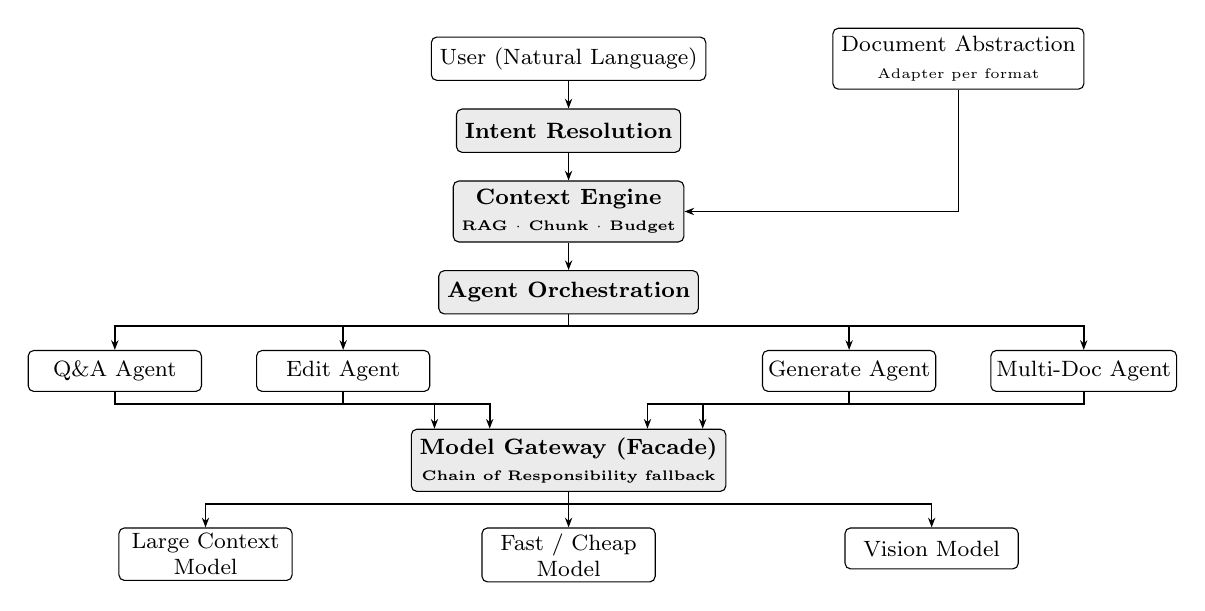
\begin{tikzpicture}[
  font=\footnotesize,
  box/.style    = {rectangle, rounded corners=2pt, draw=black, fill=white,
                   minimum width=2.6cm, minimum height=0.55cm, align=center, inner sep=3pt},
  corebox/.style= {rectangle, rounded corners=2pt, draw=black, fill=black!8,
                   minimum width=2.6cm, minimum height=0.55cm, align=center, inner sep=3pt,
                   font=\footnotesize\bfseries},
  sbox/.style   = {rectangle, rounded corners=2pt, draw=black, fill=white,
                   minimum width=2.2cm, minimum height=0.52cm, align=center, inner sep=2pt},
  arr/.style    = {-{Stealth[length=3.5pt]}, black, line width=0.6pt}
]

\node[box]     (user)   {User (Natural Language)};
\node[box]     (docabs) [right=1.6cm of user] {Document Abstraction\\{\tiny Adapter per format}};
\node[corebox] (intent) [below=0.35cm of user] {Intent Resolution};
\node[corebox] (ctx)    [below=0.35cm of intent] {Context Engine\\{\tiny RAG $\cdot$ Chunk $\cdot$ Budget}};
\node[corebox] (orch)   [below=0.35cm of ctx] {Agent Orchestration};

\node[sbox] (qa)    [below left=0.45cm and 3.0cm of orch] {Q\&A Agent};
\node[sbox] (edit)  [below left=0.45cm and 0.1cm of orch] {Edit Agent};
\node[sbox] (gen)   [below right=0.45cm and 0.8cm of orch] {Generate Agent};
\node[sbox] (multi) [below right=0.45cm and 3.7cm of orch] {Multi-Doc Agent};

\node[corebox] (gw) [below=1.45cm of orch] {Model Gateway (Facade)\\{\tiny Chain of Responsibility fallback}};

\node[sbox] (m1) [below left=0.45cm and 1.5cm of gw]  {Large Context\\Model};
\node[sbox] (m2) [below=0.45cm of gw]                  {Fast / Cheap\\Model};
\node[sbox] (m3) [below right=0.45cm and 1.5cm of gw]  {Vision Model};

\draw[arr] (user)   -- (intent);
\draw[arr] (docabs.south) -- ++(0,-1.54) |- (ctx.east);
\draw[arr] (intent) -- (ctx);
\draw[arr] (ctx)    -- (orch);

\draw[arr] (orch.south) -- ++(0,-0.15) -| (qa.north);
\draw[arr] (orch.south) -- ++(0,-0.15) -| (edit.north);
\draw[arr] (orch.south) -- ++(0,-0.15) -| (gen.north);
\draw[arr] (orch.south) -- ++(0,-0.15) -| (multi.north);

\draw[arr] (qa.south)    -- ++(0,-0.15) -| ($(gw.north west)!0.15!(gw.north)$);
\draw[arr] (edit.south)  -- ++(0,-0.15) -| ($(gw.north west)!0.50!(gw.north)$);
\draw[arr] (gen.south)   -- ++(0,-0.15) -| ($(gw.north east)!0.50!(gw.north)$);
\draw[arr] (multi.south) -- ++(0,-0.15) -| ($(gw.north east)!0.15!(gw.north)$);

\draw[arr] (gw.south) -- ++(0,-0.15) -| (m1.north);
\draw[arr] (gw)       -- (m2);
\draw[arr] (gw.south) -- ++(0,-0.15) -| (m3.north);

\end{tikzpicture}
\end{center}
\vspace{2pt}

%────────────────────────────────────────────────────────────────────
\section{Expected Time to Build a Prototype}

The team of 5 will \textbf{architect the entire system} but \textbf{implement only 2--3 end-to-end use cases}:

(1)~Grounded Document Q\&A with source citations,

(2)~Scoped AI editing with diff view and accept/reject, and

(3)~model routing across at least two LLM providers. The remaining components (multi-doc synthesis, draft generation) will be fully designed but not implemented.

\vspace{4pt}
\begin{tabular}{@{} p{3.0cm} p{1.3cm} p{9.4cm} @{}}
\toprule
\textbf{Phase} & \textbf{Duration} & \textbf{Activities} \\
\midrule
Research \& Planning   & 3 days  & Domain study, RAG framework evaluation, model API comparison, scope finalisation \\
Architecture Design    & 6 days  & Component diagrams, pattern assignments, API contracts, DB schema, interface definitions \\
Development            & 2 weeks & \textit{Stream A:} Ingestion + Context Engine.\quad \textit{Stream B:} Model Gateway + Agents.\quad \textit{Stream C:} Edit pipeline + Diff UI \\
Integration \& Testing & 4 days  & End-to-end flow tests for 3 use cases, unit + integration tests across pipeline stages \\
Refinement             & 3 days  & Bug fixes, edge-case hardening, documentation, demo preparation \\
\bottomrule
\end{tabular}
\vspace{3pt}

\noindent Total: \textbf{4 weeks}. Three parallel development workstreams with daily syncs for interface integration.

%────────────────────────────────────────────────────────────────────
\section{Domain}

\textbf{Productivity.} DocPilot directly addresses the challenge of literature synthesis, study material generation, and multi-source analysis in academic settings. The pipeline architecture is domain-agnostic by design --- with different corpora and routing policies, the same system applies to legal document review, financial analysis, and clinical research --- making the architectural contribution generalisable well beyond a single domain.

\end{document}